% !TeX document-id = {c4322337-97f4-4774-8cec-63b51c788533}
% !TeX spellcheck = en_US
% !BIB TS-program = biber
%!TEX TS-program = xelatex
\documentclass{beamer}

\usepackage{ICEF-theme/beamerthemeICEF} % Load HSE theme
\setbeamertemplate{section in toc}[sections numbered]
\setbeamertemplate{subsection in toc}[subsections numbered]

%%% Fonts 
\usepackage{fontspec}
\defaultfontfeatures{Ligatures={TeX},Renderer=Basic}
\setmainfont[Ligatures={TeX,Historic}]{Myriad Pro} % install Myriad Pro or replace with Arial
\setsansfont{Myriad Pro}  % install Myriad Pro or replace with Arial
\setmonofont{Courier New}

\usepackage{multicol} 		% Multiple columns
\newcommand*\rfrac[2]{{}^{#1}\!/_{#2}}
\usepackage{bbm}
\usepackage[style=apa,
		maxcitenames=1,
		%maxnames=10,
		url=false,
		doi=false,
		eprint=false,
		backend=biber]{biblatex}
\addbibresource{../Sources/lit.bib}

\makeatletter
\def\blfootnote{\gdef\@thefnmark{}\@footnotetext}
\makeatother

\makeatletter
\patchcmd{\beamer@sectionintoc}{\vskip1.5em}{\vskip0.5em}{}{}
\makeatother

\usepackage{multicol}
\usepackage{multirow}
\usepackage{makecell}
\usepackage{booktabs}
\usepackage[linesnumbered]{algorithm2e} %boxed

%%% Author and speech
\title[ERPT in Russia]{Determining Exchange Rate Pass-through in Russia} 
\author[Artur Zmanovskii]{Artur Zmanovskii}
\institute[ICEF]{Higher School of Economics \\ International College of Econonomics and Finance}
\date{10th June 2021}

\begin{document}	% Document begins

\frame[plain]{\titlepage}	% Title frame

%\section{Overview}
\begin{frame}
\frametitle{Overview}
\tableofcontents[hideothersubsections]
\end{frame}

\section{Introduction}
\begin{frame}
\frametitle{Introduction}
\framesubtitle{Justification}
\begin{itemize}
	\item Price stability in an open economy depends on import prices $\Rightarrow$ local price level is subject to exchange rate fluctuations;
	\item In general, there is no one-to-one correspondence: producers along the distribution chain may adjust their markup to mitigate exchange rate shock;
	\item Russia has been exposed to numerous different macroeconomic shocks, especially oil price fluctuations\\$\Rightarrow$ it is crucial to estimate shock-dependent exchange rate pass-through.
\end{itemize}
\end{frame}


\section{Literature Review}
\begin{frame}
\frametitle{Literature Review}
\framesubtitle{Russian unconditional ERPT}
\begin{itemize}
	\item Only one work \parencite{Khotulev2020} estimates shock-dependent ERPT using DSGE;
	\item Values vary from paper to paper as well as data time-frame. 
\end{itemize}
\begin{table}[h]
	\centering
	\resizebox{\textwidth}{!}{
		\begin{tabular}{llllll}
			Paper                                   & Currency & Data         & Infl. aggr. & Length    & ERPT \\
			\midrule
			\cite{Oomes2005}       & NEER               & 1996--2004   & CPI             & Short-run & 0.4--0.5     \\
			\cite{Korhonen2006} & USD & 1999--2004 & ULC\footnote{Unit labour cost.} & Long-run & -0.42 \\
			\cite{Dobrynskaya2008} & NEER               & 1995--2002   & CPI             & Long-run  & 0.35         \\
			\cite{Kataranova2010}  & USD                & 2000--2008   & CPI             & Short-run & 0.06--0.2    \\
			\cite{Beckmann2013}    & USD                & 1999--2010   & CPI             & Long-run  & -0.17        \\
			\cite{Ponomarev2016}   & NEER               & 2000--2012   & CPI             & Short-run & 0.046        \\
			\cite{Faryna2016}      & USD                & 2000--2015   & CPI Core        & Long-run  & 0.1          \\
			\cite{Sinyakov2019}    & NEER               & (2016--2017) & CPI             & Long-run  & 0.35         \\
			\cite{Khotulev2020}    & NEER               & 2005--2019   & CPI             & Long-run  & 0.16        \\
			\bottomrule
		\end{tabular}
	}
	%\caption{Earlier shock-independent ERPT estimates for Russia.}
	\label{table:litreview_erpt}
\end{table}
\end{frame}

\section{Methods}
\begin{frame}
	\frametitle{Methods}
	\framesubtitle{Definitions: unconditional ERPT}
	\begin{itemize}
		\item Basic method --- estimation of ARDL model:
		\begin{equation}
			INFL_t = \alpha_0 + \alpha_1 NEER_t + \alpha_2 NEER_{t-1} + \ldots + \beta'\gamma_t + \epsilon_t
		\end{equation}
		\item Then, unconditional exchange rate pass-through (\textbf{ERPT}) value for horizon $t$ is as follows:
		\begin{equation}
			\textstyle ERPT_h = \sum_{i=1}^{h} \alpha_i
		\end{equation}
		\item Main drawback --- ERPT value is unconditional, shock-independent --- not informative.
	\end{itemize}
\end{frame}

\begin{frame}
	\frametitle{Methods}
\framesubtitle{Definitions: shock-dependent ERPT (PERR)}
\begin{itemize}
	\item Another option is to estimate VAR (either using frequentist or Bayesian approach) and calculate price-to-exchange rate ratio (PERR, as in \textcite{Ortega2020}), for example:
	\begin{equation}
		{Y}_t = \mathbf{C} + \mathbf{B_1} Y_{t-1} + \ldots + u_t, \quad \mathbb{E}(u u') = \Sigma_u
	\end{equation}
	\begin{equation}
		Y_t = \left[\text{CPI}_t, \text{GDP}_t, \text{IR}_t, \text{ER}_t, \text{OIL}_t\right]', \; 	u_t = \left[u^{\text{CPI}}_t, \ldots, u^{\text{OIL}}_t\right]'.
	\end{equation}
	\begin{equation}
		PERR_{h,shock} = \frac{\sum_{t=1}^{h}\text{IRF}_{t,shock}^{\text{CPI}}}{\sum_{t=1}^{h}\text{IRF}_{t,shock}^{\text{ER}}},
	\end{equation}
	\item Reduced-form VAR does not capture structural shocks ($\Sigma_u$ is not diagonal) $\Rightarrow$ need to use identification scheme.
\end{itemize}
\blfootnote{ER = exchange rate, IR = interest rate, IRF = impulse response function.}
\end{frame}

\begin{frame}
		\frametitle{Methods}
	\framesubtitle{SVAR}
	\begin{itemize}
		\item Full-form VAR:
		\begin{equation}
			\mathbf{A_0}{Y}_t = \tilde{\mathbf{C}} + \mathbf{A_1} Y_{t-1} + \ldots + \epsilon_t, \quad \mathbb{E}(\epsilon \epsilon') = \Sigma_\epsilon = \mathbb{I}_n.
		\end{equation}
		$\epsilon_t = \left[\epsilon^{\text{CPI}}_t, \ldots, \epsilon^{\text{OIL}}_t\right]'$ is a vector of \textit{structural} shocks at $t$, and model captures contemporaneous relations of variables.
		\item The most common way to get matrix of structural parameters --- $A_0$ --- is to use Cholesky decomposition of covariance matrix $\Sigma_u$:
		\begin{equation}
			\Sigma_u = (A_0)^{-1} \Sigma_\epsilon (A_0)^{-1'} = (A_0)^{-1} (A_0)^{-1'}.
		\end{equation}
		\item A huge drawback --- this identification scheme is recursive (upper-/lower-triangular) $\Rightarrow$ rigid.
	\end{itemize}
\end{frame}

\begin{frame}
	\frametitle{Methods}
	\framesubtitle{Zero and sign restrictions}
	\begin{itemize}
	\item \parencite{Arias2014} proposes to use agnostic suggestions about signs and zero values of IRF to identify shocks:
	\begin{enumerate}
		\item Obtain $n$ draws from posterior distribution of BVAR;
		\item For each draw generate $m$ random matrices $X_n$ and use QR decomposition to get orthonormal matrices $Q$ such that $Q'Q = I_n$. Transform $Q$ using an algorithm described in paper, if there are zero restrictions;
		\item For each matrix $Q$ calculate $IRF_h \times Q$, where $IRF_h$ is column-stacked IRF values calculated from corresponding draw, and check whether the result satisfies zero and sign restrictions. 
	\end{enumerate}
	\item Suitable for under-identified and just-identified models;
	\item There should be less zero restrictions than an order of a particular shock.
	\end{itemize}
\end{frame}


\section{Data and model}
\subsection{Data}
\begin{frame}
\frametitle{Data}
\framesubtitle{Variables}
\begin{itemize}
	\item Quarterly data, 2005Q2--2020Q4, 63 observations;
	\item All variables, except for interest rate, are in growth rates;
	\item Two CPI aggregates: full and core (excl. fuel, fruits and vegetables, community transport services, utilities etc.).
\end{itemize}
\begin{table}[b!]
	\centering
	\resizebox{\textwidth}{!}{%
	\begin{tabular}{@{}lll@{}}
		\toprule
		Variable  & Description  & Source    \\ \midrule
		Oil price & \makecell[l]{Brent oil price nominated in US dollars, \\quarterly average, QoQ.} & Bloomberg \\
		Interest rate & \makecell[l]{MIACR 31--180 days, quarterly average.}& CBR        \\
		Exchange rate & \makecell[l]{Nominal effective exchange rate (NEER) of ruble, \\Ruble appreciation = NEER decline, \\QoQ, Central Bank of Russia methodology.} & CBR        \\
		Output        & \makecell[l]{Russian real GDP (2015Q1 = 100), \\seasonally adjusted by institution, QoQ.}  & \makecell[l]{FRED} \\
		Price level & \makecell[l]{Consumer price index and core consumer price index, QoQ, \\seasonally adjusted (X13-SEATS), Rosstat methodology.}          & Rosstat   \\ \bottomrule
	\end{tabular}%
	}
	%\caption{Description of Data and Sources}
	\label{table:variables_decription}
\end{table}
\end{frame}

\subsection{Model}
\begin{frame}
\frametitle{Model}
\framesubtitle{Identification scheme}
\begin{itemize}
	\item Two 1-lag BVAR specifications: full and core CPI for price level variable. Order is chosen based on SIC criterion. Conjugate normal inverse-Wishart prior is used;
	\item 500 draws from posterior distribution, 1000 random $Q$ matrices for each draw;
	\item Restriction scheme is based on \parencite{Forbes2018} and \parencite{Sinyakov2019};
	\item Sign restrictions are for contemporaneous and next quarter reaction, zero restrictions are only contemporaneous.
	\begin{table}[h!]
		\centering
		\resizebox{0.9\textwidth}{!}{%
			\begin{tabular}{@{}lccccc@{}}
				\toprule
				Variable & \makecell{Demand \\shock} & \makecell{Supply \\shock} & \makecell{Monetary \\shock} & \makecell{Exchange rate \\shock} & \makecell{Global persistent \\shock} \\
				\midrule
				CPI/Core & +   & --   & -- & + & ?   \\
				Real GDP  & + & +   & -- & ? & ?   \\
				Interest rate & +   & ?   & +   & + & ?   \\
				NEER          & ?   & ? & -- & + & -- \\
				Oil price     & 0   & 0   & 0   & 0 & +  \\
				\bottomrule
			\end{tabular}%
		}
		\label{tab:signs_and_zeros}
	\end{table}
\end{itemize}
\end{frame}

\section{Results}
\begin{frame}
\frametitle{Results}
\framesubtitle{PERR}
\begin{itemize}
	\item Almost all PERR values for core composition are higher;
	\item Exchange rate shock pass-through is the highest in LR for both specifications;
	\item Global shock PERR is low for full CPI and huge for core composition;
	\item Supply shock PERRs are comparable for both specifications;
	\item Except for supply shock, pass-through is faster for core CPI.
\end{itemize}
\begin{table}[h!!]
	\centering
	\small
	\resizebox{0.75\textwidth}{!}{%
	\begin{tabular}{@{}lcccc@{}}
		\toprule
		Horizion& \multicolumn{2}{c}{Short-run (1Q)} & \multicolumn{2}{c}{Long-run (4Q)} \\
		\midrule
		Shock                   & \makecell[c]{PERR\\(CPI)}      & \makecell[c]{PERR\\(Core)}      & \makecell[c]{PERR\\(CPI)}      & \makecell[c]{PERR\\(Core)}     \\
		\midrule
		Global persistent shock & 0.070          & 0.344           & 0.158          & 0.427          \\
		Monetary shock          & 0.044          & 0.110           & 0.281          & 0.448          \\
		Exchange rate shock     & 0.146         & 0.197           & 0.403          & 0.565         \\
		Supply shock            & -0.239         & -0.124          & -0.356         & -0.391          \\ % & -0.2389         & -0.0239          & -0.3556         & -0.3907         \\
		Demand shock            & -0.037         & -0.295          & -0.133         & -0.354   \\
		\bottomrule
	\end{tabular}%
	}
	%\caption{\small PERR calculated for BVAR with sign and zero restrictions. ''CPI'' and ''core'' in parentheses reflect price aggregate (CPI or Core CPI) used in the model.}
	\label{tab:perr}
\end{table}
\end{frame}

\begin{frame}
\begin{figure}[h!]
	\centering
	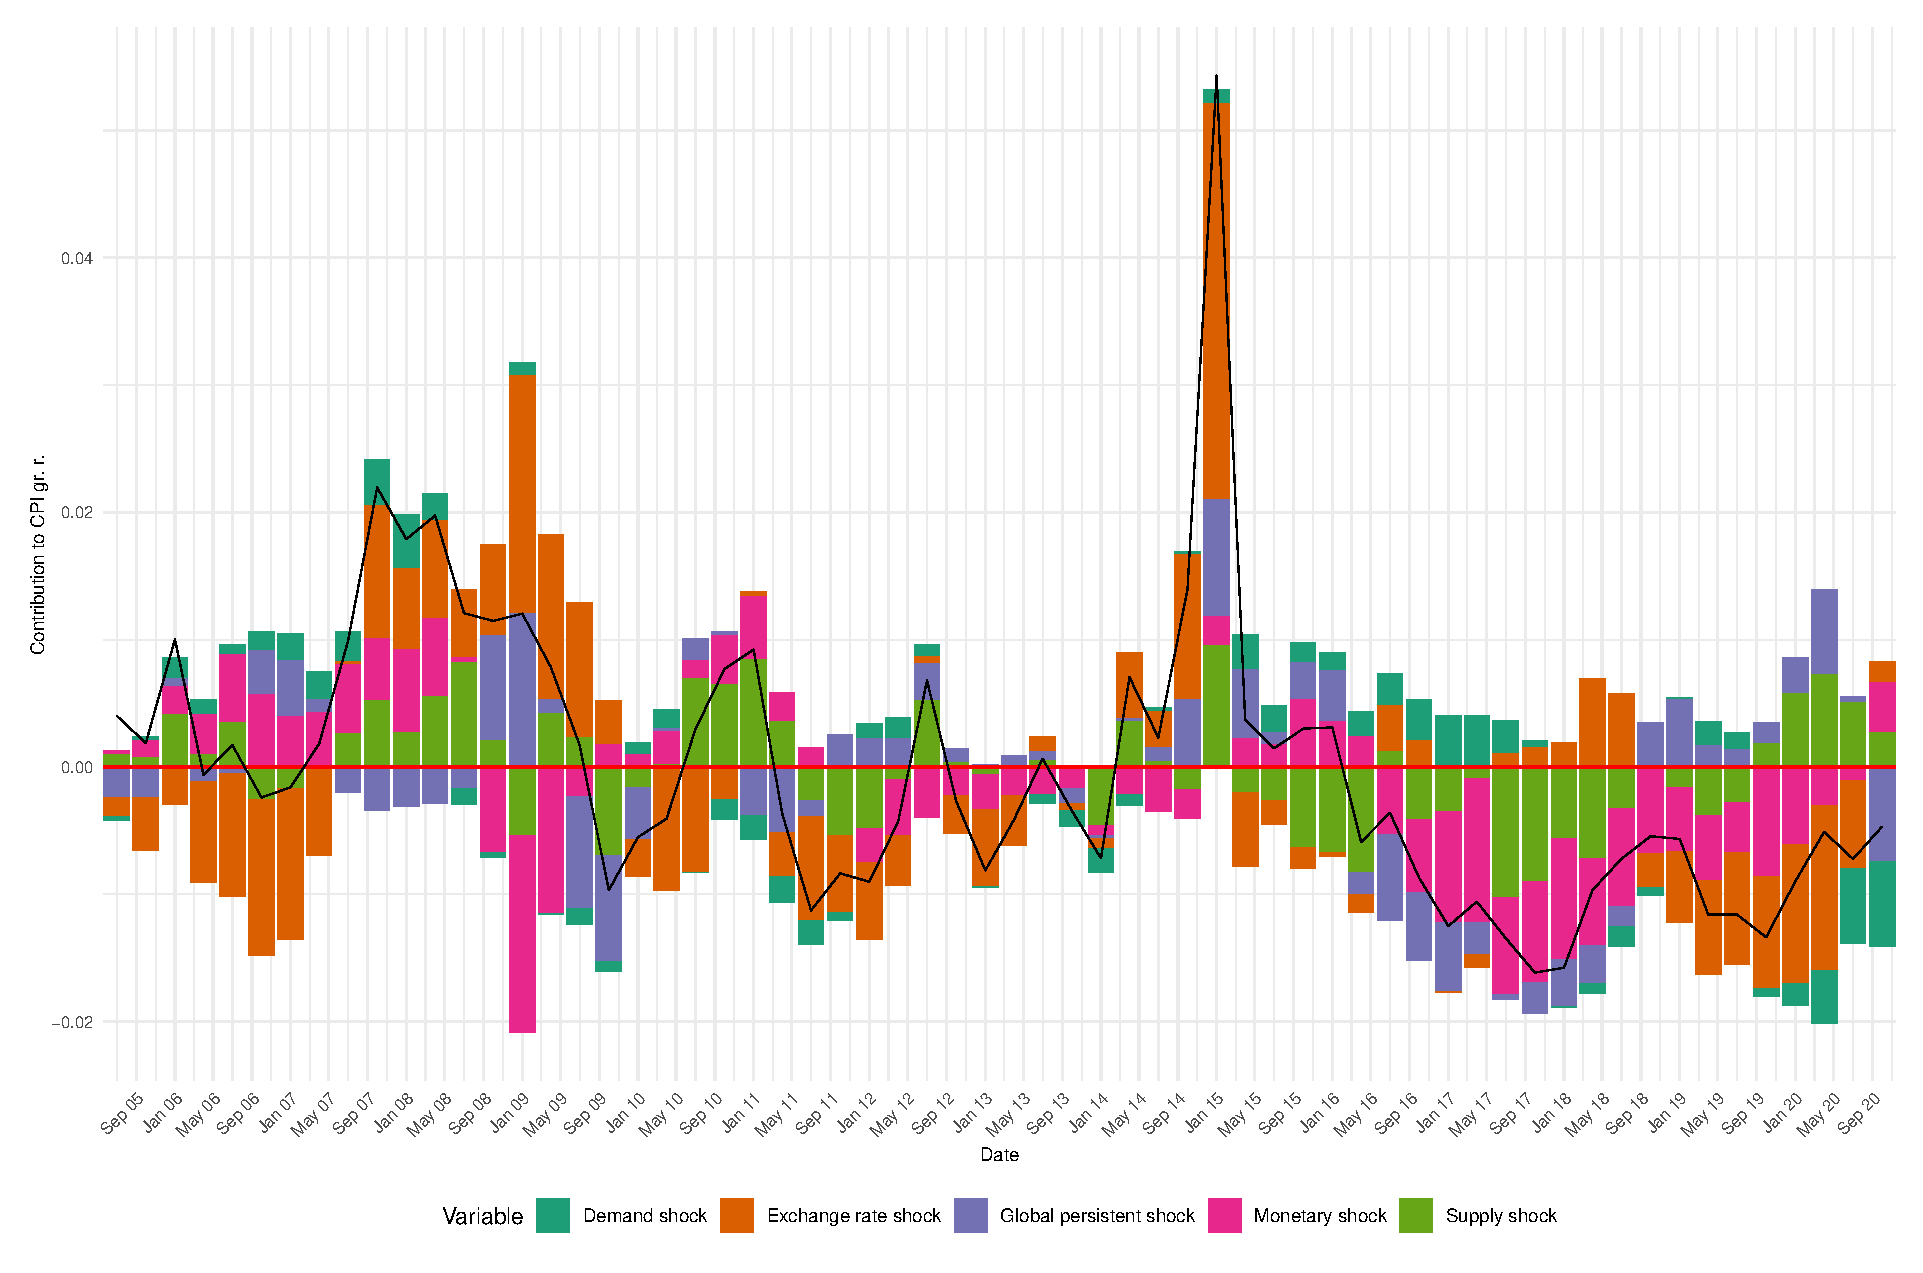
\includegraphics[width=1\linewidth]{../Text/figures/hd_cpi_full}
	\caption[]{Hist. decomp. of demeaned CPI gr. r. time series.}
	\label{fig:hd_cpi_full}
\end{figure}
\end{frame}

\section{Conclusion}
\begin{frame}
\frametitle{Conclusion}
	\begin{itemize}
		\item Result is comparable to \parencite{Khotulev2020} for monetary and global shocks;
		\item PERR values are higher for Russia comparing to Euro area;
		\item Exchange rate pass-through is higher and faster to core CPI;
		\item COVID-19 crisis has been driven mainly by global persistent and demand shocks;
		\item Policy implications: 
		\begin{enumerate}
			\item Pass-through during exogenous ER shock is high, more aggressive exchange rate management may be beneficial;
			\item Monetary policy vs. domestic supply trade-off: positive monetary shock cools down both prices and output in SR, but may be a source of negative supply shocks in LR.
		\end{enumerate}
	\end{itemize}
\end{frame}

\begin{frame}
	\frametitle{Q\&A}
	\label{qa}
	\begin{columns}
		\begin{column}{0.49\textwidth}
			\tableofcontents[hideothersubsections]
		\end{column}
		\begin{column}{0.49\textwidth}
			\begin{itemize}
				\item \hyperlink{software}{Software discussion}
				\item \hyperlink{zero_q}{How is Q matrix constructed with zero restrictions?}
				\item \hyperlink{bvar}{Bayesian model specification}
				\item \hyperlink{time_series}{Data plot}, \hyperlink{intrate_cpi}{Interest~rate~vs.~inflation~plot}
				\item \hyperlink{fullirfs}{Full CPI IRFs},  \hyperlink{coreirfs}{Core CPI IRFs}
				\item \hyperlink{corehd}{Core CPI HD}
			\end{itemize}
		\end{column}
	\end{columns}
\end{frame}

\appendix
\section{Annex}
\begin{frame}[noframenumbering]{Annex}
\framesubtitle{Software discussion}
	\label{software}
	\begin{enumerate}
		\item Matlab --- \href{https://eeecon.uibk.ac.at/~breitenlechner/data/ZeroSignVAR.zip}{\texttt{ZeroSignVAR}}:
		\begin{itemize}
			\item No long-run IRFs;
			\item Bug with hist. dec. figures --- some colors are erroneously identical. 
		\end{itemize}
		\item R --- \href{https://cran.r-project.org/package=BVAR}{\texttt{BVAR}}:
			\begin{itemize}
			\item No long-run IRFs;
			\item Only contemporaneous restrictions;
			\item No historical decomposition. 
		\end{itemize}
		\item Eviews --- \href{https://www.eviews.com/Addins/arw.aipz}{\texttt{arw}}:
		\begin{itemize}
			\item No long-run IRFs;
			\item Rigid restrictions.
		\end{itemize}
		\item R --- \href{https://github.com/roootra/ZerosignR}{\texttt{ZerosignR}} --- my implementation, which implements long-run IRF restrictions. \textit{Under development}.
	\end{enumerate}
	\hyperlinkpresentationend{\beamerreturnbutton{Return to Q\&A}}
\end{frame}

\begin{frame}[noframenumbering]{Annex}
	\framesubtitle{Zero restrictions on Q matrix}
	\label{zero_q}
	\begin{algorithm}[H]
		\KwData{$Z$ = zero restrictions matrix, $n$ = number of zero restrictions, $Z_j$ = $j$-th shock zero restrictions, $1 \le j \le n$, $z_j$ = number of zero restrictions for shock $j$ such that $z_j \le n-j$. $R_j(A_0, A_+) = \begin{bmatrix}
			Z_j \times IRF(A_0, A_+)\\
			Q'_{j-1} \end{bmatrix}$. $Q_{j} = \left[q_1, \ldots, q_j\right]'$, $q_j$ = $j$-th column of $Q$, $Q_0 = q_0 \equiv \emptyset$.}
		\For{$j=1 \ldots n$}{
			$N_{j-1} = \text{Null}(R_j)$;\\
			$x_j \sim \mathbb{N}_{n}(0,1)$;\\
			$q_j = N_{j-1}\frac{N'_{j-1}x_j}{\parallel N'_{j-1}\parallel}$;
		}
	\end{algorithm}
	\begin{itemize}
		\item Zero restrictions are held by construction.
	\end{itemize}
	\hyperlinkpresentationend{\beamerreturnbutton{Return to Q\&A}}
\end{frame}

\begin{frame}[noframenumbering]{Annex}
	\framesubtitle{Bayesian model}
	\label{bvar}
	\begin{itemize}
		\item Conjugate normal-inverse Wishart distribution for BVAR (underline for prior values):
		\begin{equation}
			\begin{cases}
					\Sigma \sim \mathcal{IW}(\underline{S}, \underline{\nu})\\
					\mathbf{B} | \Sigma  \sim \mathcal{N} (\underline{\mathbf{B}}, \Sigma \otimes (X'X))
				\end{cases}
		\end{equation}
		\begin{itemize}
			\item $\Sigma$ = error covariance matrix, $\mathcal{IW}$ = inverse-Wishart distribution, $S$ = scale matrix (pos. def.) of $\mathcal{IW}$, $\nu$ = degrees of freedom;
			\item $\mathbf{B}$ = matrix of coefficients, $\mathcal{N}$ = normal multivariate distribution, $X$ = matrix of regressors (columns of lagged $Y$), $\otimes$ = Kronecker product;
			\item No need for Gibbs sampler and burn-in --- parameters are derived analytically;
			\item Can use initial $\Sigma$ from OLS.
		\end{itemize}
	\end{itemize}
	\hyperlinkpresentationend{\beamerreturnbutton{Return to Q\&A}}
\end{frame}

\begin{frame}[noframenumbering]{Annex}
	\framesubtitle{Reception of reviews}
	\label{reception}
	\begin{enumerate}
		\item \textit{Why didn't I estimate unconditional ERPT?}
		\begin{itemize}
			\item Shock-dependent ERPT (PERR) is not studied well for Russia;
			\item Unconditional ERPT requires discussion about specification of model and choice of data --- a whole separate dissertation would have been written;
		\end{itemize}
		\item \textit{Why didn't I split time series to periods before/after adoption of floating regime?}
		\begin{itemize}
			\item 24 quarterly observations after Bank of Russia's decision to adopt floating regime --- few for estimation of VAR, even using Bayesian approach.
		\end{itemize}
		\item \textit{Why don't I capture adoption effect using a separate shock?}
		\begin{itemize}
			\item Quite unclear how to do that in SVAR framework;
			\item Shock vs. structure problem: can be addressed by estimating threshold VAR or TVP-VAR, but identification is cumbersome, and there are no works solving this issue.
			%\item Need to add additional variable to the model, while pursuing parsimony;
			%\item Chicken and egg problem: introducing a shock to understand reaction of macro variables, while needing guessing the signs of the shock to identify it;
		\end{itemize}
	\end{enumerate}
\hyperlinkpresentationend{\beamerreturnbutton{Return to Q\&A}}  \hyperlinkslidenext{\beamergotobutton{ERPT estimation}}
\end{frame}

\begin{frame}[noframenumbering]{Annex}
	\hypertarget{uncerpt}{}
	\framesubtitle{ERPT estimation}
	\begin{itemize}
		\item À-la \parencite{Campa2005} --- ARDL model with NEER as exchange rate, GDP and oil as proxies:
	\begin{equation}
		CPI_t = c + \sum_{i=0}^4 \alpha_i NEER_{t-i} + \sum_{i=0}^2 \beta_i GDP_{t-i}  + \sum_{i=0}^2 \gamma_i OIL_{t-i} + \varepsilon_t.
	\end{equation}
		\item Short-run (2Q) ERPT: $\sum_{i=0}^1 \beta_i = 0.199$ (p<0.0001);
		\item Long-run (4Q) ERPT: $\sum_{i=0}^3 \beta_i = 0.272$ (p<0.0001);
		\item Roughly speaking, LR ERPT is half as much as LR PERR for any shock.
	\end{itemize}
	\hyperlinkpresentationend{\beamerreturnbutton{Return to Q\&A}}
\end{frame}

\begin{frame}[noframenumbering]
	\label{corehd}
	\begin{figure}[h!]
		\centering
		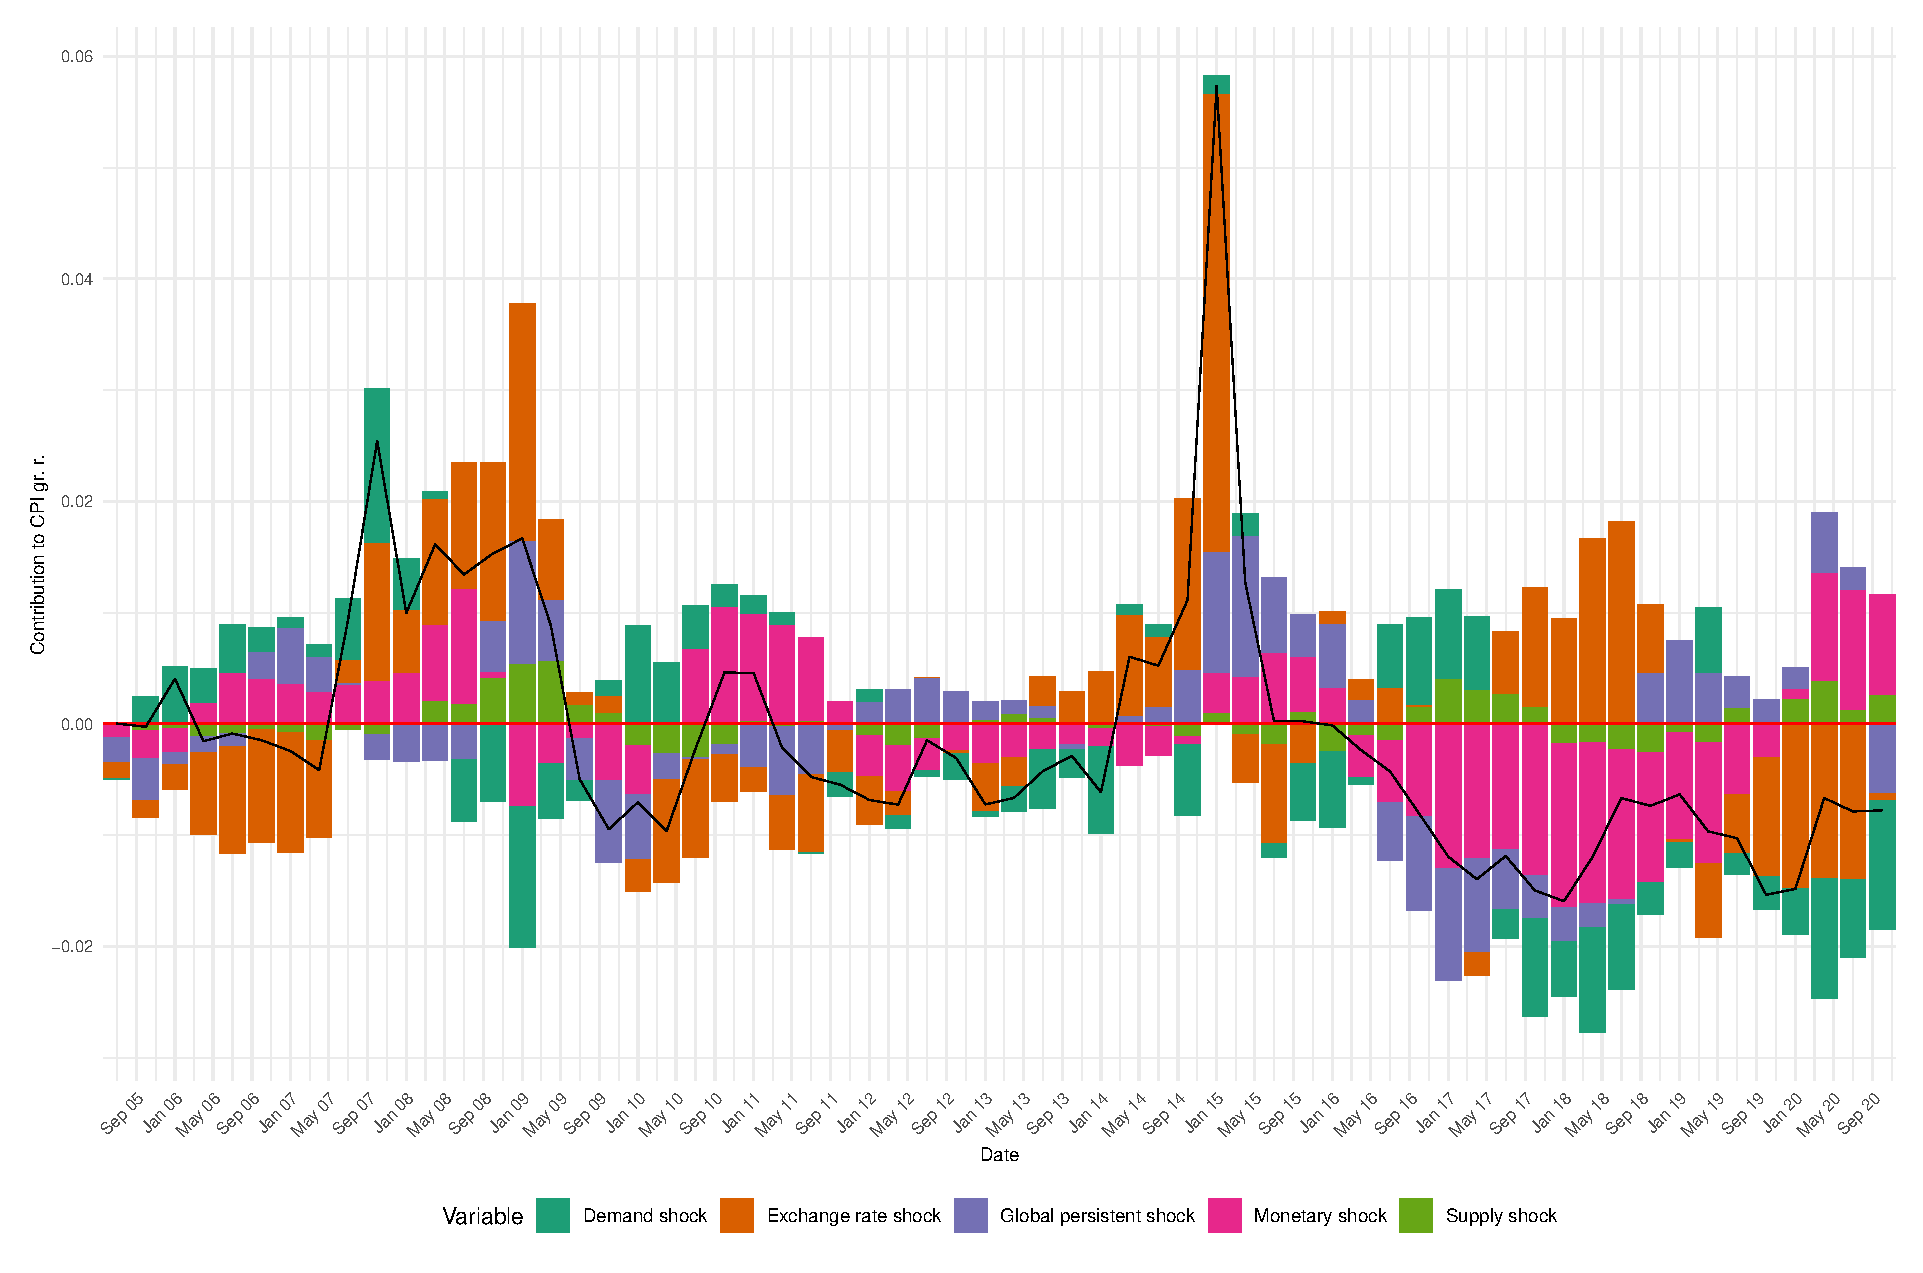
\includegraphics[width=1\linewidth]{../Text/figures/hd_core_cpi_full}
		\caption[]{Hist. decomp. of demeaned NEER gr. r. time series, core CPI.}
		\label{fig:hd_cpi_core}
	\end{figure}
	\hyperlinkpresentationend{\beamerreturnbutton{Return to Q\&A}}
\end{frame}

\begin{frame}[noframenumbering]
	\label{intrate_cpi}
	\begin{figure}[h!]
		\centering
		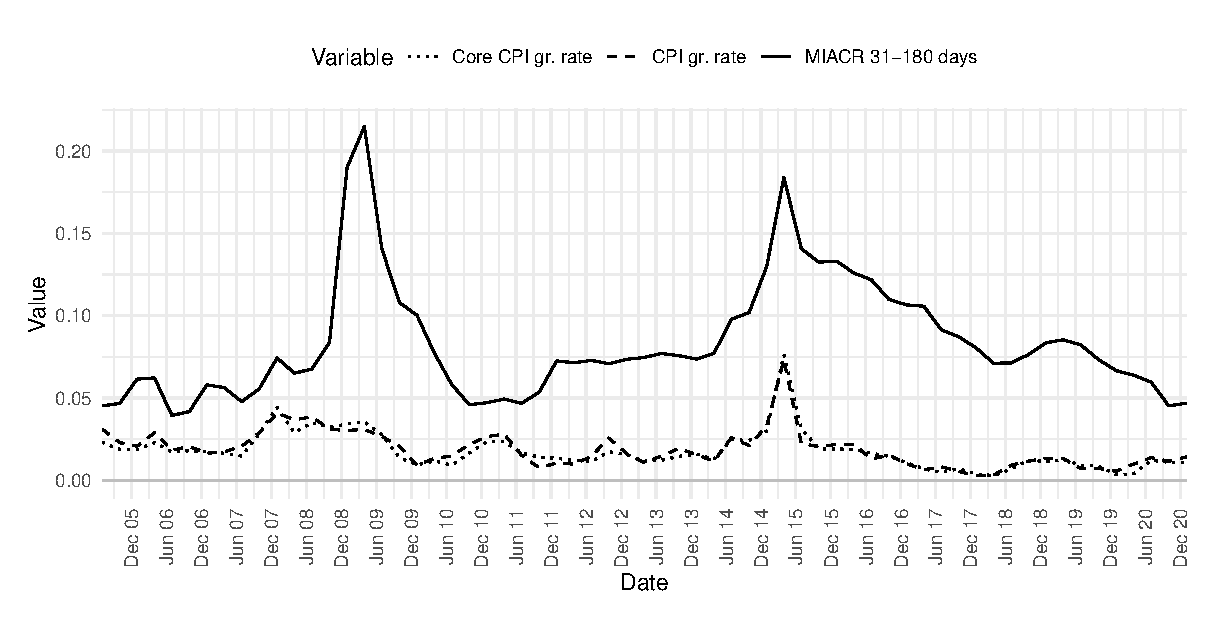
\includegraphics[width=1\linewidth]{../Text/figures/intrate_cpi}
		\caption[]{Time series of interest rate and growth rates of full and core CPI compositions.}
		\label{fig:intrate_cpi}
	\end{figure}
	\hyperlinkpresentationend{\beamerreturnbutton{Return to Q\&A}}
\end{frame}

\begin{frame}[noframenumbering]
	\label{time_series}
	\begin{figure}[h!]
		\centering
		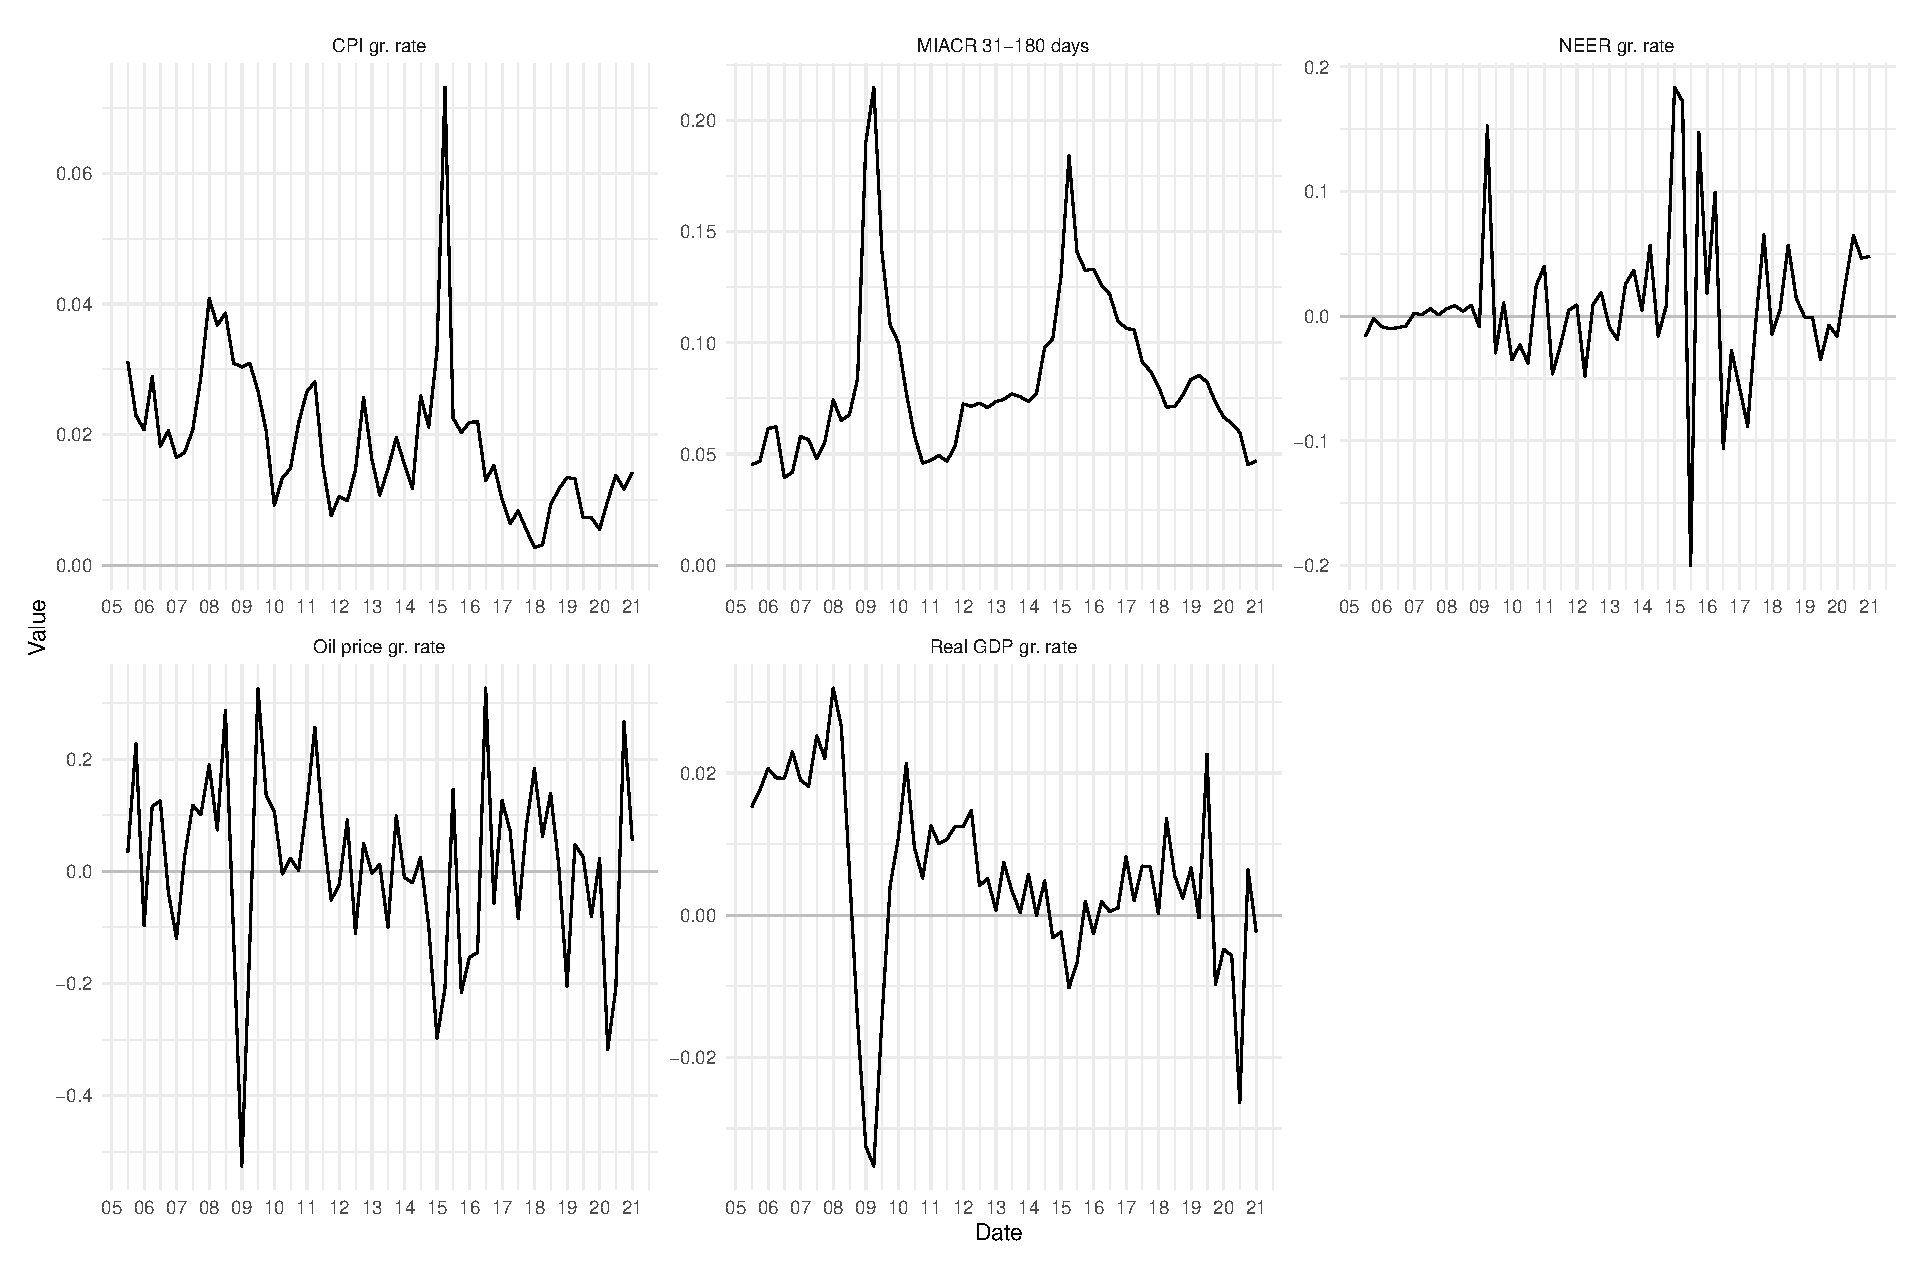
\includegraphics[width=1\linewidth]{../Text/figures/time_series}
		\caption[]{Time series of variables used, growth rates except for interest rate.}
		\label{fig:time_series}
	\end{figure}
	\hyperlinkpresentationend{\beamerreturnbutton{Return to Q\&A}}
\end{frame}

\begin{frame}[noframenumbering]
	\label{fullirfs}
	\begin{figure}[h!]
		\centering
		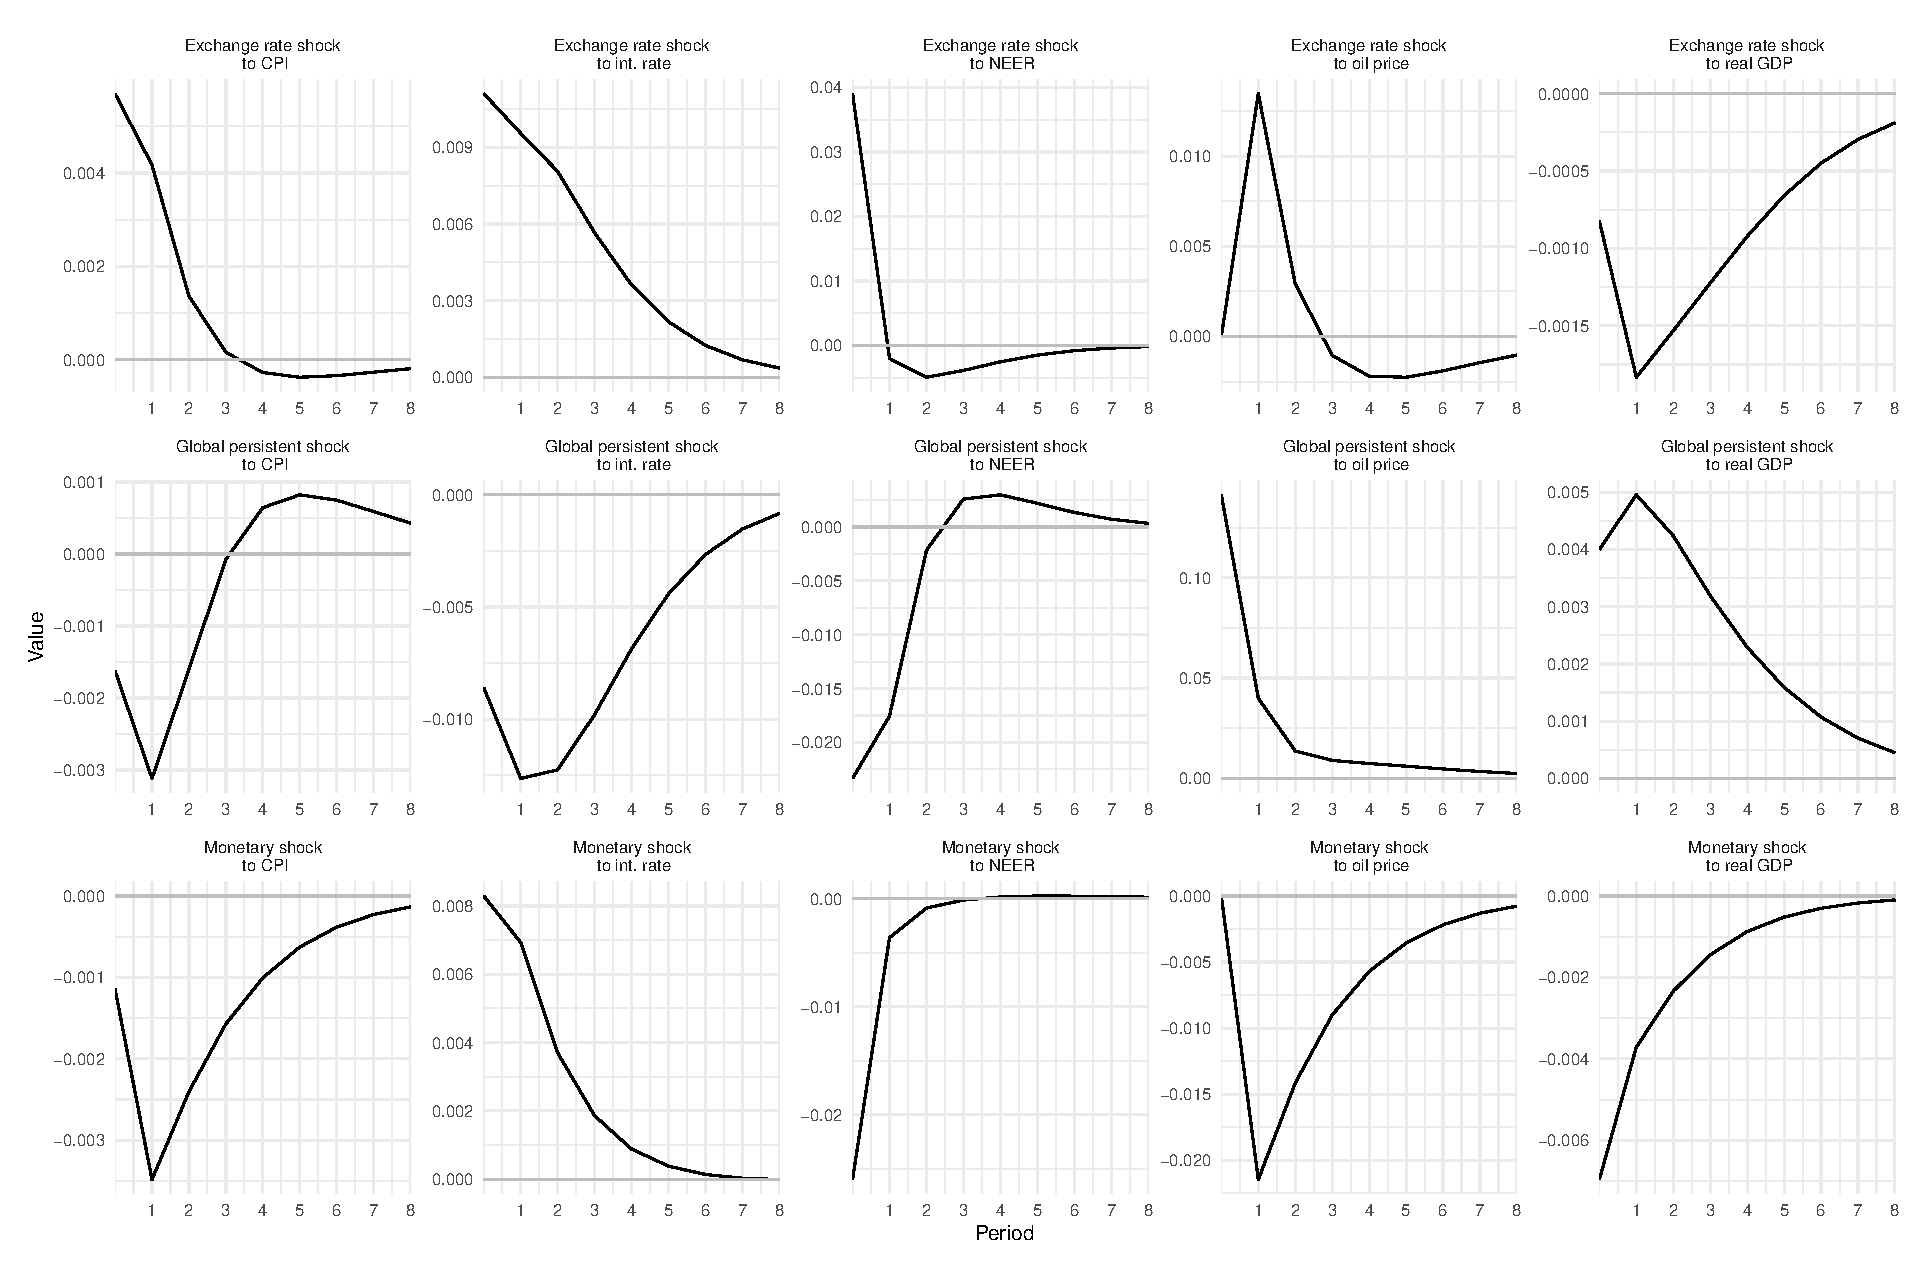
\includegraphics[width=1\linewidth]{../Text/figures/irf_1}
		\caption[]{Impulse response functions of full model, CTM (1).}
		\label{fig:irf_1}
	\end{figure}
\hyperlinkpresentationend{\beamerreturnbutton{Return to Q\&A}} \hyperlinkslidenext{\beamergotobutton{Continue...}}
\end{frame}

\begin{frame}[noframenumbering]
	\begin{figure}[h!]
		\centering
		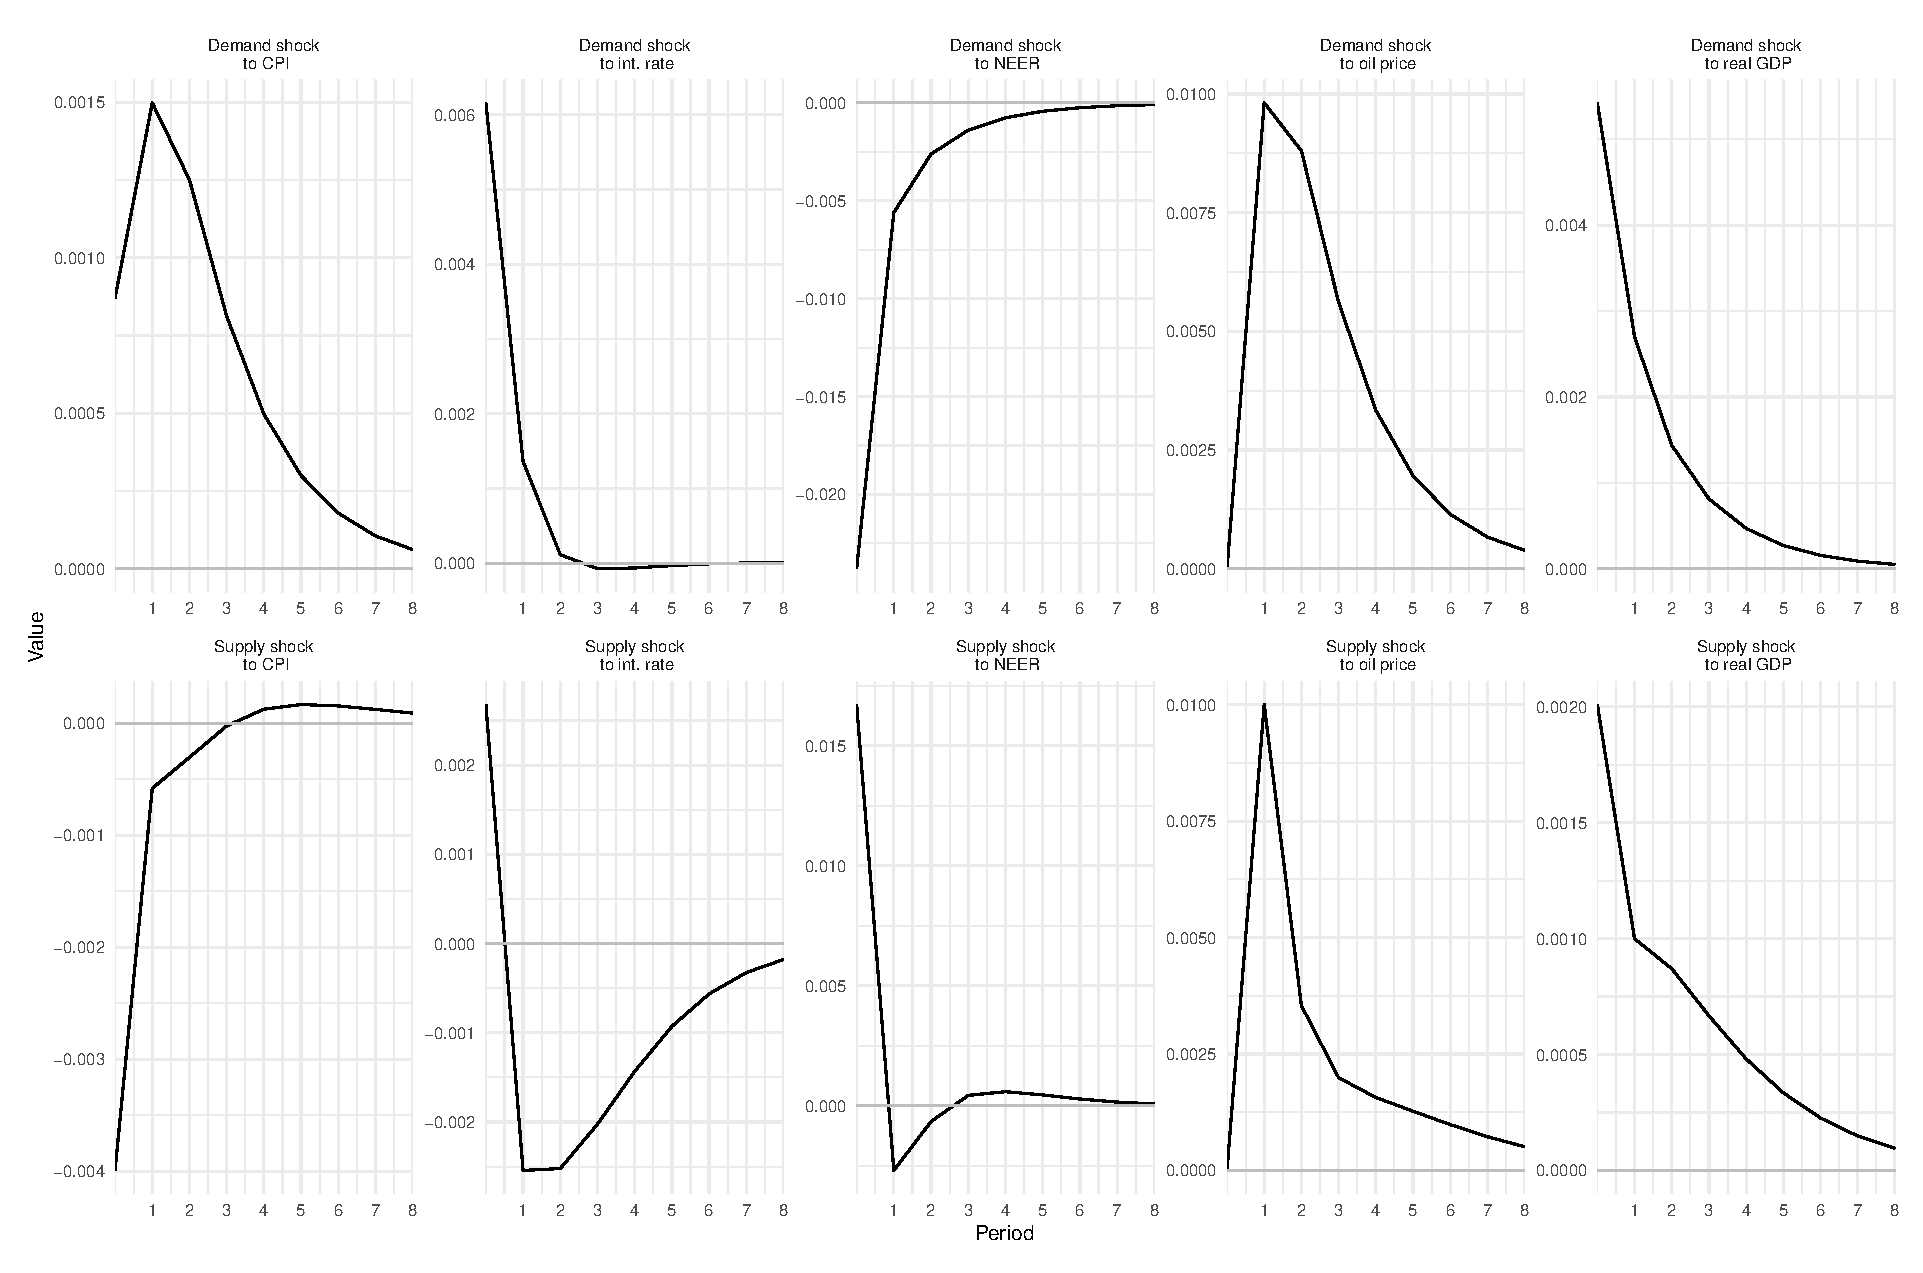
\includegraphics[width=1\linewidth]{../Text/figures/irf_2}
		\caption[]{Impulse response functions of full model, CTM (2).}
		\label{fig:irf_2}
	\end{figure}
\hyperlinkpresentationend{\beamerreturnbutton{Return to Q\&A}}
\end{frame}

\begin{frame}[noframenumbering]
	\label{coreirfs}
	\begin{figure}[h!]
		\centering
		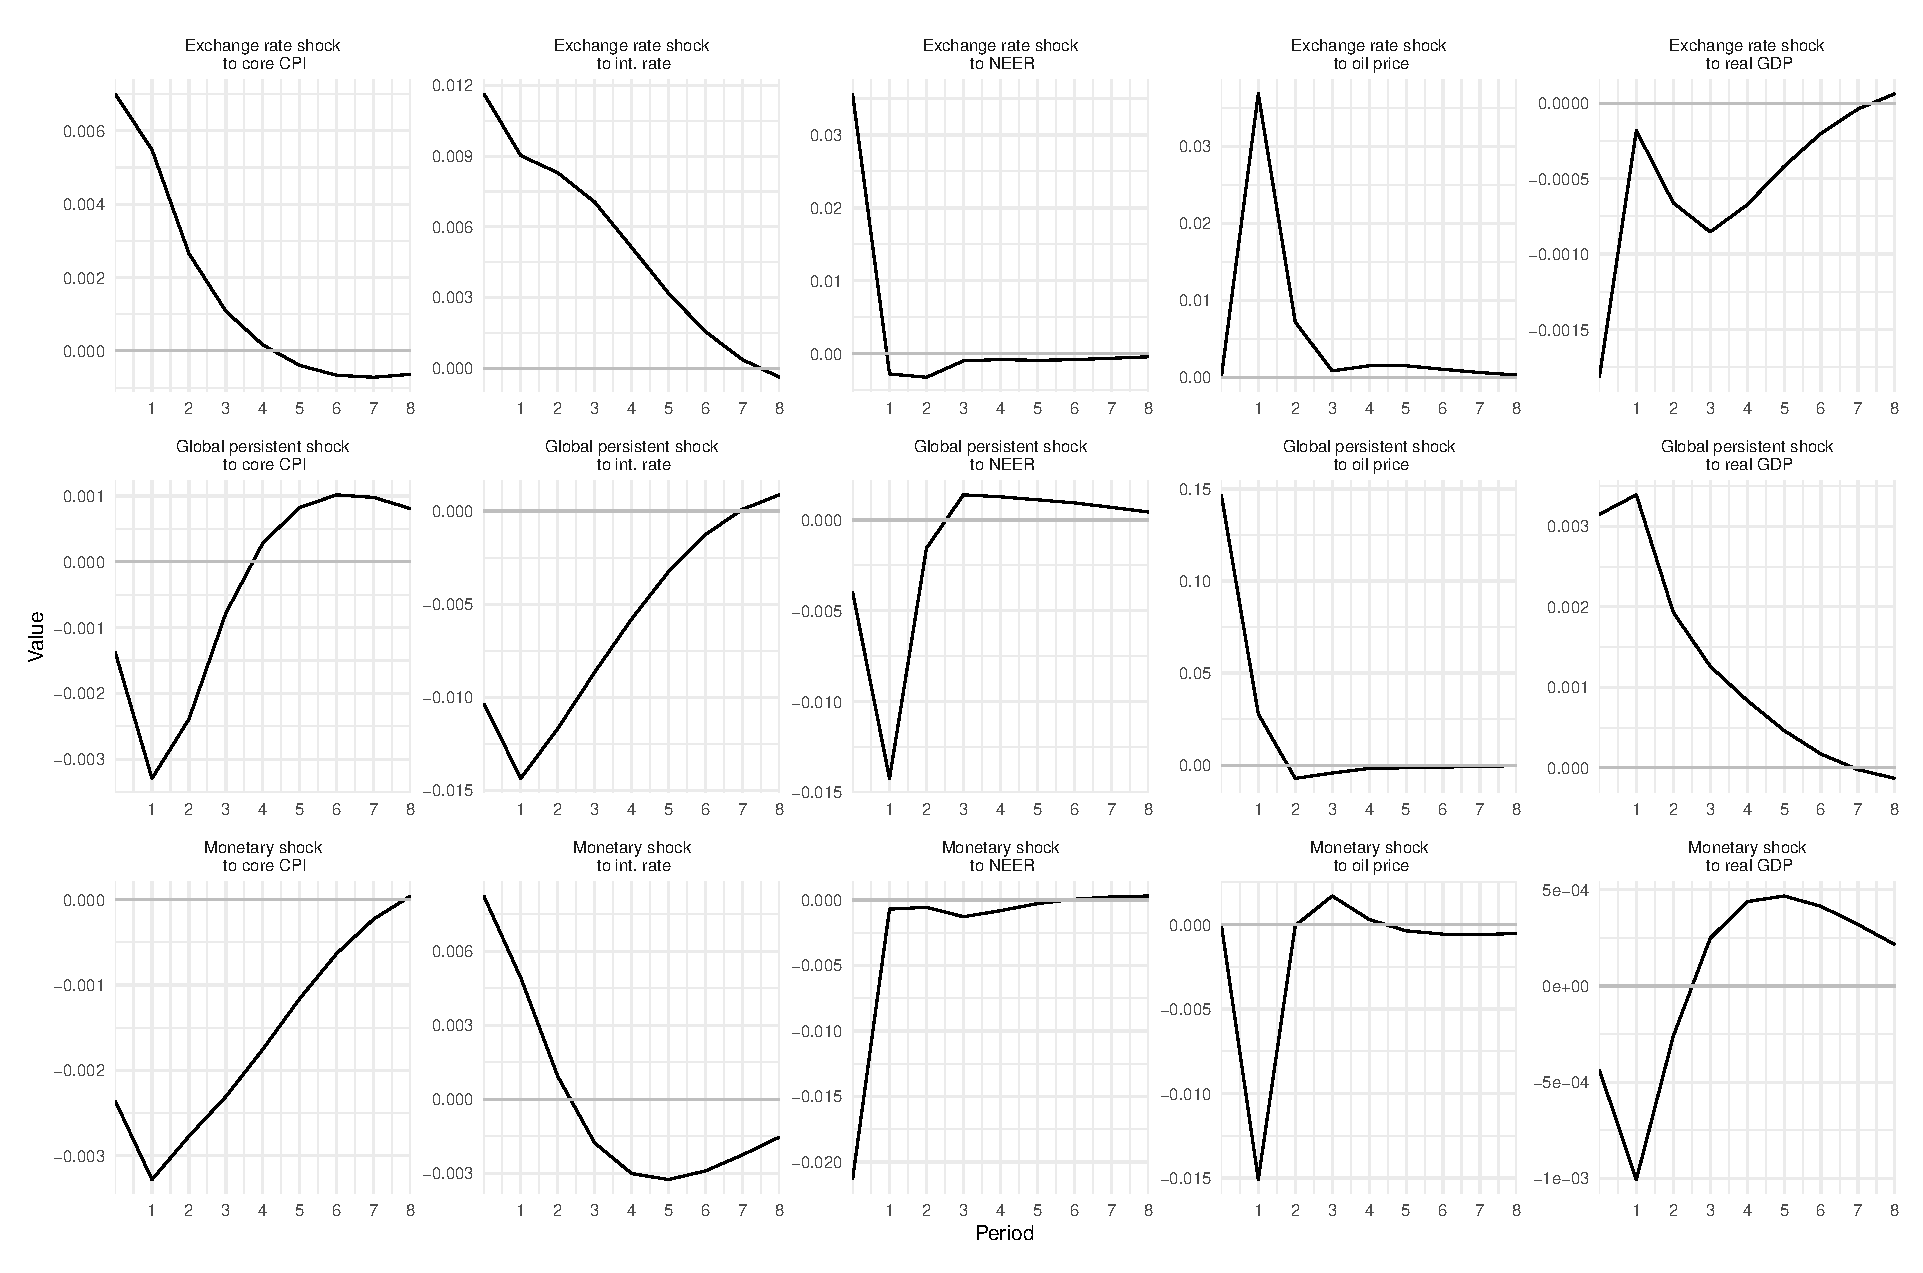
\includegraphics[width=1\linewidth]{../Text/figures/irf_core_1}
		\caption[]{Impulse response functions of core model, CTM (1).}
		\label{fig:irf_core_1}
	\end{figure}
\hyperlinkpresentationend{\beamerreturnbutton{Return to Q\&A}} \hyperlinkslidenext{\beamergotobutton{Continue...}}
\end{frame}

\begin{frame}[noframenumbering]
	\begin{figure}[h!]
		\centering
		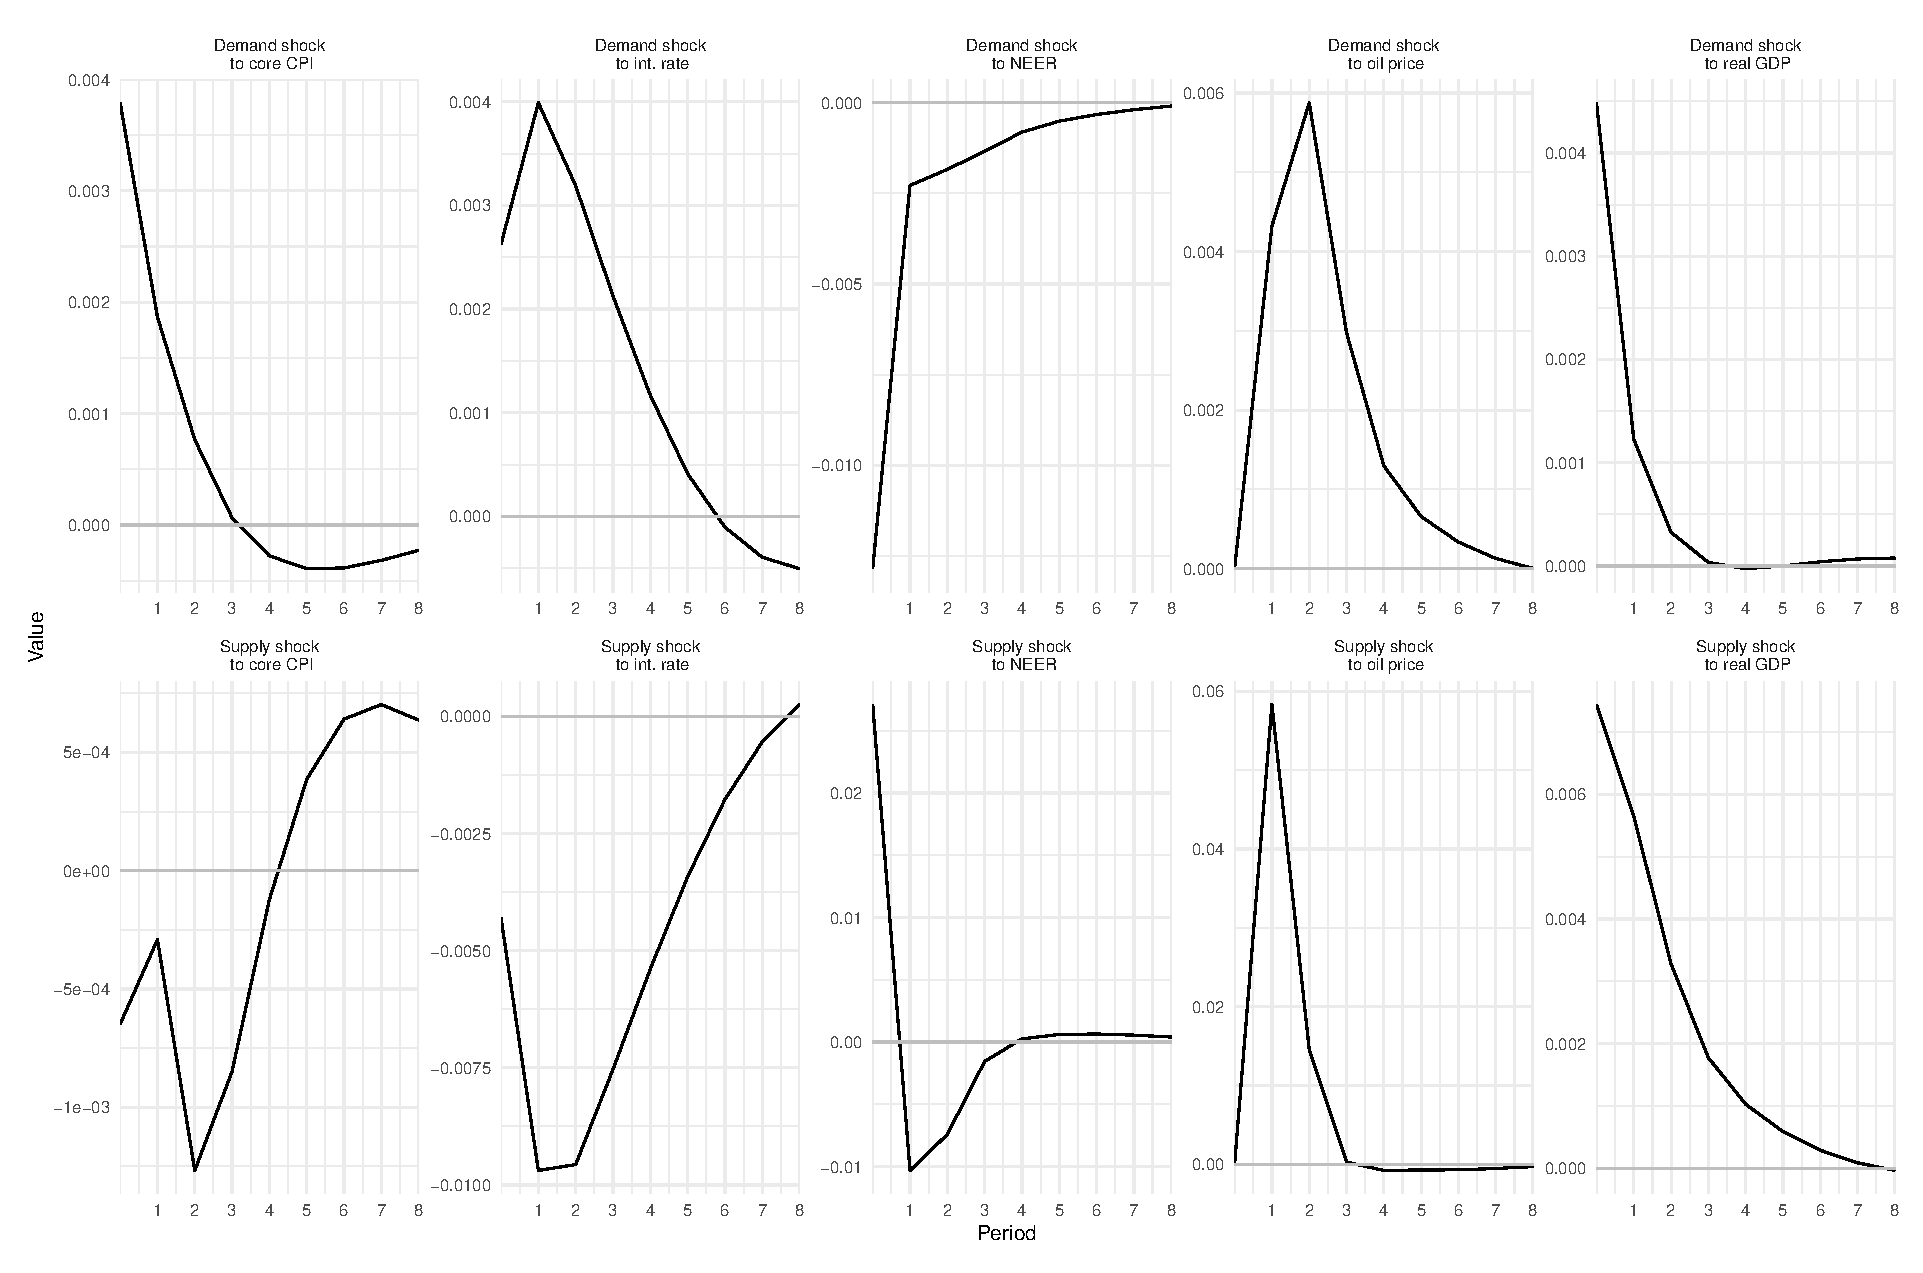
\includegraphics[width=1\linewidth]{../Text/figures/irf_core_2}
		\caption[]{Impulse response functions of core model, CTM (2).}
		\label{fig:irf_core_2}
	\end{figure}
\hyperlinkpresentationend{\beamerreturnbutton{Return to Q\&A}}
\end{frame}

\begin{frame}[noframenumbering, allowframebreaks]
	\frametitle{References}
	\label{references}
	\tiny{
		\printbibliography[heading=none]}
\end{frame}

\end{document}